%%%%%%%%%%%%%%%%%%%%%%%%%%%%%%%%%%%%%%%%%%%%%%%%%%%%%%%%%%%%%%%%%%%%%%%%%%%%%%%%
% DEFINE DOCUMENT TYPE
%%%%%%%%%%%%%%%%%%%%%%%%%%%%%%%%%%%%%%%%%%%%%%%%%%%%%%%%%%%%%%%%%%%%%%%%%%%%%%%%
\documentclass[11pt, oneside]{mnthesis}


%%%%%%%%%%%%%%%%%%%%%%%%%%%%%%%%%%%%%%%%%%%%%%%%%%%%%%%%%%%%%%%%%%%%%%%%%%%%%%%%
% IMPORT PACKAGES
%%%%%%%%%%%%%%%%%%%%%%%%%%%%%%%%%%%%%%%%%%%%%%%%%%%%%%%%%%%%%%%%%%%%%%%%%%%%%%%%
\usepackage{epic,eepic,units}
\usepackage{hyperref}
\usepackage{url}

% From:
% http://tex.stackexchange.com/questions/12703/how-to-create-fixed-width-table-columns-with-text-raggedright-centered-raggedlef
\usepackage{array}
\newcolumntype{L}[1]{>{\raggedright\let\newline\\\arraybackslash\hspace{0pt}}p{#1}}
\newcolumntype{C}[1]{>{\centering\let\newline\\\arraybackslash\hspace{0pt}}p{#1}}
\newcolumntype{R}[1]{>{\raggedleft\let\newline\\\arraybackslash\hspace{0pt}}p{#1}}

%\usepackage{longtable}
%\usepackage{mathrsfs}
%\usepackage{multirow}
%\usepackage{bigstrut}
%\usepackage{amssymb}
%\usepackage{graphicx}
\usepackage{cite}
\usepackage{paralist}
\usepackage[stable]{footmisc}   %Lets us use footnotes in section headers.
% \usepackage[style={square, numbers}]{natbib}
% \usepackage{amsmath}
% \usepackage{amssymb}
% \usepackage{amsthm}
% \usepackage{caption}
% \usepackage[vertfit]{breakurl}
\usepackage{listings, multicol}
\usepackage{enumitem}
\usepackage{subcaption}  % subfigures
\usepackage{bibentry}
% \usepackage[section, numberedsection=autolabel, nonumberlist]{glossaries}

%Dealing with dutch names:
% http://tex.stackexchange.com/questions/40747/bibtex-handling-of-the-dutch-van-name-prefix-with-natbib
\DeclareRobustCommand{\VAN}[2]{#2}
\usepackage {graphicx}
\usepackage[cmex10]{amsmath}
\usepackage{amssymb}
\usepackage{stmaryrd}
\usepackage{amsthm}
\usepackage{algorithmic}
\usepackage{array}
%\usepackage{mdwmath}
%\usepackage{mdwtab}
\usepackage{eqparbox}
%\usepackage[tight,normalsize]{subfigure}
%\usepackage[font=normalsize]{caption}
%\usepackage{tabularx,colortbl}
\usepackage[dvipsnames]{xcolor}
\usepackage{flushend}
\usepackage{cite}
\usepackage{amsmath}
%\usepackage[font=footnotesize]{subfig}
%\usepackage[caption=false,font=footnotesize]{subfig}
\usepackage{fixltx2e}
\usepackage[ruled, vlined, linesnumbered]{algorithm2e}
\usepackage{stfloats}
\usepackage{url}
\usepackage{xspace}
\theoremstyle{definition}
\hyphenation{op-tical net-works semi-conduc-tor}
\newcommand{\mkeyword}[1]{\mbox{\texttt{#1}}}
\DeclareMathOperator{\kuop}{uop}
\DeclareMathOperator{\kbop}{bop}
\DeclareMathOperator{\kite}{ite}
\DeclareMathOperator{\kpre}{pre}
\DeclareMathOperator{\dom}{dom}
\DeclareMathOperator{\ktrue}{true}
\DeclareMathOperator{\kfalse}{false}
\DeclareMathOperator{\kselect}{select}
\DeclareMathOperator{\ran}{range}
\newcommand{\lbb}{[\![}
\newcommand{\rbb}{]\!]}
\newcommand{\expr}{\phi}
\newcommand{\exprS}{\Phi}

\definecolor{gold}{rgb}{0.90,.66,0}
\definecolor{dgreen}{rgb}{0,0.6,0}
\newcommand{\mike}[1]{\textcolor{red}{#1}}
\newcommand{\fixed}[1]{\textcolor{purple}{#1}}
\newcommand{\andrew}[1]{\textcolor{green}{#1}}
\newcommand{\ela}[1]{\textcolor{blue}{#1}}
\newcommand{\stateequiv}{\equiv_{s}}
\newcommand{\traceequiv}{\equiv_{\sigma}}
\newcommand{\ta}{\text{TA}}
\newcommand{\cta}{\text{TA$_{C}$}}
\newcommand{\tta}{\text{TA$_{T}$}}

\newcommand{\bfalg}{\texttt{\small{IVC\_BF}}}
\newcommand{\ucalg}{\texttt{\small{IVC\_UC}}}
\newcommand{\ucbfalg}{\texttt{\small{IVC\_UCBF}}}
\newcommand{\mustalg}{\texttt{\small{IVC\_MUST}}}

\newcommand{\nondetcov}{\text{\sc Nondet-Cov}}
\newcommand{\nondetcovalt}{\text{\sc Nondet-Cov$^{*}$}}
\newcommand{\ivccov}{\text{\sc IVC-Cov}}
\newcommand{\maycov}{\text{\sc May-Cov}}
\newcommand{\mustcov}{\text{\sc Must-Cov}}
\newcommand{\allcov}{\text{\sc Model-Cov}}
\newcommand{\mutcov}{\text{\sc Mutant-Cov}}


\newtheorem{lemma}{Lemma}
\newtheorem{definition}{Definition}
\newtheorem{coroll}{Corollary}
\newtheorem{theorem}{Theorem}
\newtheorem{note}{Note}

%%%%%%%%%%%%%%%%%%%%%%%%%%%%%%%%%%%%%%%%%%%%%%%%%%%%%%%%%%%%%%%%%%%%%%%%%%%%%%%%
% ADDITIONAL PREABLE MATERIAL
%%%%%%%%%%%%%%%%%%%%%%%%%%%%%%%%%%%%%%%%%%%%%%%%%%%%%%%%%%%%%%%%%%%%%%%%%%%%%%%%
\hypersetup{
    colorlinks,
%     %Set the link colors.
%     citecolor=black,
%     filecolor=blue,
%     linkcolor=blue,
%     urlcolor=blue
    %To turn off color, comment out the block above and uncomment the block
    % below.
    citecolor=black,
    filecolor=black,
    linkcolor=black,
    urlcolor=black
}

% Suppresses inline citation page numbers if they are defined using \cite.
    \let\oldcite\cite
    \renewcommand\cite[2][]{\oldcite{#2}}

% \setcounter{secnumdepth}{5}

% % \appendix{Glossary}
% \begin{description}
% \item[process]\label{def:process}  ``set of interrelated or interacting
%     activities which transforms inputs into outputs''~\cite{_iso9000_2005}
% \item[work package]\label{def:work_package}  small pieces of functionality or
%     supporting documentation to be completed
% \end{description}

\newglossaryentry{def:brownfield_project}
{
    name={brownfield project},
    description={a project that is based on or must coexist with one or more
            legacy systems} 
}

\newglossaryentry{def:challenged_project}
{
    name={challenged project},
    description={a project that completes ``late, over-budget, and/or with less
            than required features or functions''~\cite[p.1]{_chaos_2013}; with
            agile techniques, typically only schedule and cost concerns are
            measured} 
}


\newglossaryentry{def:failed_project}
{
    name={failed project},
    description={a project that was unable to complete because it was 
        ``cancelled prior to completion or delivered and never 
        used''~\cite[p.1]{_chaos_2013}} 
}


\newglossaryentry{def:greenfield_project}
{
    name={greenfield project},
    description={a project that is not constrained by any prior work, such as
            legacy systems} 
}

\newglossaryentry{def:method-family}
{
    name={method-family},
    description={the process type; a group of processes that can be
        characterized by a set of well-defined properties (e.g., agile,
        traditional)},
    plural={method-families}
}


\newglossaryentry{def:oracle}
{
    name={oracle},
    description={the standard by which we can compare the output of a
        system being evaluated} 
}


\newglossaryentry{def:process}
{
    name=process,
    description={``set of interrelated or interacting
                activities which transforms inputs into
                outputs''~\cite{_iso9000_2005}},
    user1={_iso9000_2005},
    plural=processes 
}


\newglossaryentry{def:process_characterization}
{
    name={process characterization},
    description={determining the properties of the project and product to be
        completed and establishing the project's goals (such as focusing on
        quality)~\cite{xu_using_2008}}
}


\newglossaryentry{def:process_model}
{
    name={process model},
    description={an abstraction of a process; this may be either a model that
        represents a concrete process or a pre-tailored form of a model (e.g.,
        scrum, extreme programming, spiral model)}
}


\newglossaryentry{def:project_network}
{
    name={project network},
    description={the set of \glspl{def:work_package} and their
        interdependencies}
}


\newglossaryentry{def:successful_project}
{
    name={successful project},
    description={a completed project that was ``delivered on time, on budget,  
        with required features and functions''~\cite[p.1]{_chaos_2013}}
}


\newglossaryentry{def:triple_constraint}
{
    name={triple-constraint},
    description={a set of metrics---cost, schedule, and scope (including
        quality)---commonly used to evaluate project success; also a method for
        balancing project priorities (limiting one of the metrics results in
        changes---increased cost, increased schedule, and decreased scope---in
        one or both of the other constraints)} 
}


\newglossaryentry{def:work_breakdown_structure}
{
    name={work breakdown structure},
    description={}
}


\newglossaryentry{def:work_package}
{
    name={work package},
    description={small pieces of functionality or supporting documentation to be
                 completed}
}





% 
% 
%     \item[High-level Process Model Selection]  Select the high-level process
%             model (e.g. Scrum or XP for the agile method-family) as the basis
%             for further specialization.
%     \item[Tailoring]  Adapting the process model to meet the
%             specific needs or constraints of the organization, product, and
%             project.
%     \item[Process Evaluation (Verification and Validation)]  Verifying and
%         validating that the process (or process model instance) meets the needs
%         of the team and is ``consistent with the project goals and
%         environment''~\cite{xu_using_2008}.  This can be performed in a number
%         of ways.
%             \textbf{TODO -- this part should be its own (sub)section.}
%     \item[Adoption (Execution)]  Implementing the process within the
%             organization to complete the project.  Depending on the process,
%             this may involve \textit{in~situ} process analysis and improvements.
%     \item[Post-mortem Analysis]  Evaluating the process after it has been
%             executed to improve later projects.
% \makeglossaries

% %%%%%%%%%%%%%%%%%%%%%%%%%%%%%%%%%%%%%%%%%%%%%%%%%%%%%%%%%%%%%%%%%%%%%%%%%%%%%%%%
% Custom definitions
%%%%%%%%%%%%%%%%%%%%%%%%%%%%%%%%%%%%%%%%%%%%%%%%%%%%%%%%%%%%%%%%%%%%%%%%%%%%%%%%
\newcommand{\C}{{\mathrm{c}}}

\newcommand{\COS}{{\mathrm{cos}}}
\newcommand{\SIN}{{\mathrm{sin}}}
\newcommand{\DOF}{{\mathrm{dof}}}
\newcommand{\MSEC}{\mu{\mathrm{s}}}
\newcommand{\NS}{\mathrm{ns}}
\newcommand{\PPM}{{\mathrm{ppm}}}
\newcommand{\ENR}{{\mathrm{GeV}}}
\newcommand{\MOM}{{\mathrm{GeV/c}}}

\newcommand{\CONT}{\noindent}
\newcommand{\FIG}{Fig.\ }
\newcommand{\FIGS}{Figs.\ }
\newcommand{\SEC}{Sec.\ }
\newcommand{\SECS}{Secs.\ }
\newcommand{\TAB}{Table }
\newcommand{\TABS}{Tables }
\newcommand{\EQ}{Eq.\ }
\newcommand{\EQS}{Eqs.\ }
\newcommand{\APP}{Appendix }
\newcommand{\APPS}{Appendices }
\newcommand{\CHP}{Chapter }
\newcommand{\CHPS}{Chapters }

\newcommand{\OFF}{\emph{G2off}~}
\newcommand{\TOO}{\emph{G2Too}~}
%%%%%%%%%%%%%%%%%%%%%%%%%%%%%%%%%%%%%%%%%%%%%%%%%%%%%%%%%%%%%%%%%%%%%%%%%%%%%%%%


% FROM:
% http://tex.stackexchange.com/questions/4297/how-to-place-a-full-citation-in-the-abstract-using-bibtex
% \newcommand{\ignore}[1]{}
% \newcommand{\nobibentry}[1]{{\let\nocite\ignore\bibentry{#1}}}
% % apsrev entries in the text need definitions of these commands
% \newcommand{\bibfnamefont}[1]{#1}
% \newcommand{\bibnamefont}[1]{#1}
\nobibliography*

%%%%%%%%%%%%%%%%%%%%%%%%%%%%%%%%%%%%%%%%%%%%%%%%%%%%%%%%%%%%%%%%%%%%%%%%%%%%%%%%
% STRUCTURE SET-UP
%%%%%%%%%%%%%%%%%%%%%%%%%%%%%%%%%%%%%%%%%%%%%%%%%%%%%%%%%%%%%%%%%%%%%%%%%%%%%%%%
\newcommand{\apriori}{\textit{a~priori} }
\newcommand{\Apriori}{\textit{A~priori} }


\linespread{1.3}

%%%%%%%%%%%%%%%%%%%%%%%%%%%%%%%%%%%%%%%%%%%%%%%%%%%%%%%%%%%%%%%%%%%%%%%%%%%%%%%%
% BEGIN DOCUMENT
%%%%%%%%%%%%%%%%%%%%%%%%%%%%%%%%%%%%%%%%%%%%%%%%%%%%%%%%%%%%%%%%%%%%%%%%%%%%%%%%
\begin{document}

%%%%%%%%%%%%%%%%%%%%%%%%%%%%%%%%%%%%%%%%%%%%%%%%%%%%%%%%%%%%%%%%%%%%%%%%%%%%%%%%
% title.tex - Set up the beginning of thesis.
%%%%%%%%%%%%%%%%%%%%%%%%%%%%%%%%%%%%%%%%%%%%%%%%%%%%%%%%%%%%%%%%%%%%%%%%%%%%%%%%
% For a  PhD give the command \phd. Default is masters
%\degree (normally Doctor of Philosophy or Master of Science)
%\initials (normally Ph.D. or M.S.)
%\ms % use if for a Master of Science thesis
\phd % use if for a Ph.D. dissertation
% \draft
\topicProposaltrue

\title{\textbf{Inductive Validity Cores for Formal Verification}}
\author{Elaheh Ghassabani}
\campus{University of Minnesota}
\program{Computer Science and Engineering}
% \degree{Doctor of Philosophy}
\director{Micael W. Whalen and Mats P. E. Heimdahl}

% Optionally specify the month and year.
\submissionmonth{Oct} % defaults to current month.
\submissionyear{2017} % defaults to current year.

%Comment out below on final copy
\abstract{%Increasing usage of computer systems in safety-critical applications demands the utmost care in their specification, design, and implementation.  Formal verification is a useful method for mathematical/systematic examination of the requirements a system must meet. However, due to the complexity of modern systems, safety analysis is challenging. One of the most successful and powerful methods for formal verification is symbolic model checking.
Symbolic model checkers are useful tools for the purpose of hardware/software verification that can construct proofs of properties over
very complex models. However, the results reported by the tool
when a proof succeeds do not generally provide much insight to
the user. It is often useful for users to have traceability information related to the proof: which portions of the model were necessary to construct it.  This traceability information can be used to diagnose a variety of modeling problems such as overconstrained axioms and underconstrained properties, and can also be used to measure {\em completeness} of a set of requirements over a model.

We propose the notion of {\em inductive validity cores} (IVCs), which are intended to trace a property to a \emph{minimal} set of model elements necessary for proof. Besides minimality, computing \emph{all} minimal IVCs of a given property is
an interesting problem that provides several useful analyses, including
regression analysis for testing/proof, determination of the minimum (as
opposed to minimal) number of model elements necessary for proof, the
diversity examination of model elements leading to proof, and analyzing fault
tolerance.
%We, fisrt, propose a method to efficiently compute a single IVC within a model necessary for inductive proofs of safety properties for sequential systems.  The algorithm is based on the UNSAT core support built into current SMT solvers and a novel encoding of the inductive problem to try to generate a minimal inductive validity core.
%Then, we propose an efficient method for finding \emph{all minimal} IVCs of a
%given property. Finally, we introduce several useful applications of this idea.
%We prove our algorithms are correct, and describe their implementation in the JKind model checker for Lustre models.
%We then present an experiment in which we benchmark the algorithms in terms of speed, diversity of produced cores, and minimality, with promising results.
}
%\words{331}    % number of words in the abstract
%\copyrightpage % Do you want copyright protection?
%\acknowledgements{This thesis is a milestone in four joyful years of work with amazing UMN Critical Systems Group (CriSys). My experience at UMN has been nothing short of spectacular. Since my first day on August 20th, 2014 I have felt at home at UMN with meeting my warm-hearted and caring advisors and friends. I have been given unique opportunities and taken
advantage of them. This includes being part of the cutting-edge projects while serving as a graduate research assistant at CriSys, attending a lot of top-tier conferences, meeting with the best researchers in my field, and on top of all, learning from many distinguished and knowledgeable professors at UMN. I would like to extend thanks to the many people who so generously contributed to the work presented in this thesis.

Special mention goes to my enthusiastic supervisor, Michael Whalen. My PhD has been an amazing experience and I thank Michael, not only for his tremendous academic support, but also for giving me so many wonderful opportunities. I would like to express my sincere gratitude to him for the continuous support of my Ph.D study and related research, for his patience, motivation, and immense knowledge.

Similar, profound gratitude goes to Mats Heimdahl, who has been a truly supportive co-advisor. I am particularly indebted to him for his constant faith in my work and for his support. I have very fond memories of my time with Michael and Mats, who have been like my family all these years. Their guidance helped me in all the time of research and writing of this thesis. I could not have imagined having a better advisor and mentor for my graduate studies.

Besides my advisors, I would like to thank the rest of my thesis committee: Prof. Stephen McCamant, Prof. Marc Riedel, and Prof. Eric Van Wyk, for their insightful comments and encouragement to widen my research from various perspectives.

I thank my fellow labmates for the stimulating discussions, for the sleepless nights we were working together before deadlines, and for all the fun we have had in the last four years. Also I thank the wonderful people in other organizations I had the opportunity to work with; in particular, I am grateful to Dr. Andrew Gacek and Jaroslav Bendik.

Last but not least, I would like to thank my loving family: my parents and my sisters for supporting me spiritually throughout writing this thesis and my my life in general. }
\acknowledgements{This thesis is a milestone in four joyful years of work with amazing UMN Critical Systems Group (CriSys). My experience at UMN has been nothing short of spectacular. Since my first day on August 20th, 2014 I have felt at home at UMN with meeting my warm-hearted and caring advisors and friends. I have been given unique opportunities and taken
advantage of them. This includes being part of the cutting-edge projects while serving as a graduate research assistant at CriSys, attending a lot of top-tier conferences, meeting with the best researchers in my field, and on top of all, learning from many distinguished and knowledgeable professors at UMN. I would like to extend thanks to the many people who so generously contributed to the work presented in this thesis.

Special mention goes to my enthusiastic supervisor, Michael Whalen. My PhD has been an amazing experience and I thank Michael, not only for his tremendous academic support, but also for giving me so many wonderful opportunities. I would like to express my sincere gratitude to him for the continuous support of my Ph.D study and related research, for his patience, motivation, and immense knowledge.

Similar, profound gratitude goes to Mats Heimdahl, who has been a truly supportive co-advisor. I am particularly indebted to him for his constant faith in my work and for his support. I have very fond memories of my time with Michael and Mats, who have been like my family all these years. Their guidance helped me in all the time of research and writing of this thesis. I could not have imagined having a better advisor and mentor for my graduate studies.

Besides my advisors, I would like to thank the rest of my thesis committee: Prof. Stephen McCamant, Prof. Marc Riedel, and Prof. Eric Van Wyk, for their insightful comments and encouragement to widen my research from various perspectives.

I thank my fellow labmates for the stimulating discussions, for the sleepless nights we were working together before deadlines, and for all the fun we have had in the last four years. Also I thank the wonderful people in other organizations I had the opportunity to work with; in particular, I am grateful to Dr. Andrew Gacek and Jaroslav Bendik.

Last but not least, I would like to thank my loving family: my parents and my sisters for supporting me spiritually throughout writing this thesis and my my life in general. }
% \dedication{\input{dedication}}

% Use a special preface
%\extra{\chapter*{Author Declaration}
 \addcontentsline{toc}{chapter}{Author Declaration}
Some of the material presented within has previously been published in the
following papers:

\begin{itemize}
  \item \bibentry{de_silva_reference_2015}
\end{itemize}

\flushleft
All the work contained within represents the original contribution of the
author.}

% The \beforepreface command actually causes insertion of the title,
% abstract, signature, and copyright pages into the new document.
\beforepreface

% Define the text to go before the table of contents
\figurespage
\tablespage

% The \afterpreface command actually causes insertion of the
% contents, list of figures, etc. into the new document.
\afterpreface
%%%%%%%%%%%%%%%%%%%%%%%%%%%%%%%%%%%%%%%%%%%%%%%%%%%%%%%%%%%%%%%%%%%%%%%%%%%%%%%%





%%%%%%%%%%%%%%%%%%%%%%%%%%%%%%%%%%%%%%%%%%%%%%%%%%%%%%%%%%%%%%%%%%%%%%%%%%%%%%%%
% CONTENT
%%%%%%%%%%%%%%%%%%%%%%%%%%%%%%%%%%%%%%%%%%%%%%%%%%%%%%%%%%%%%%%%%%%%%%%%%%%%%%%%
% Input the sectons here using \input{fileName}
%%%
%\input{draft3}
% %Increasing usage of computer systems in safety-critical applications demands the utmost care in their specification, design, and implementation.  Formal verification is a useful method for mathematical/systematic examination of the requirements a system must meet. However, due to the complexity of modern systems, safety analysis is challenging. One of the most successful and powerful methods for formal verification is symbolic model checking.
Symbolic model checkers are useful tools for the purpose of hardware/software verification that can construct proofs of properties over
very complex models. However, the results reported by the tool
when a proof succeeds do not generally provide much insight to
the user. It is often useful for users to have traceability information related to the proof: which portions of the model were necessary to construct it.  This traceability information can be used to diagnose a variety of modeling problems such as overconstrained axioms and underconstrained properties, and can also be used to measure {\em completeness} of a set of requirements over a model.

We propose the notion of {\em inductive validity cores} (IVCs), which are intended to trace a property to a \emph{minimal} set of model elements necessary for proof. Besides minimality, computing \emph{all} minimal IVCs of a given property is
an interesting problem that provides several useful analyses, including
regression analysis for testing/proof, determination of the minimum (as
opposed to minimal) number of model elements necessary for proof, the
diversity examination of model elements leading to proof, and analyzing fault
tolerance.
%We, fisrt, propose a method to efficiently compute a single IVC within a model necessary for inductive proofs of safety properties for sequential systems.  The algorithm is based on the UNSAT core support built into current SMT solvers and a novel encoding of the inductive problem to try to generate a minimal inductive validity core.
%Then, we propose an efficient method for finding \emph{all minimal} IVCs of a
%given property. Finally, we introduce several useful applications of this idea.
%We prove our algorithms are correct, and describe their implementation in the JKind model checker for Lustre models.
%We then present an experiment in which we benchmark the algorithms in terms of speed, diversity of produced cores, and minimality, with promising results.

\chapter{Introduction}
\label{ch:intro}
Computer systems have become an integral part of our daily life and are being used in various environments (such as homes, hospitals, factories) and application areas (such as medical devices, aircraft flight control, weapons, and nuclear systems) where failure could lead to loss of life, financial loss, or environmental damage. The increasing reliance of critical applications on information processing makes it vital to verify the soundness and safety of the computer systems. To ensure that such software works in all cases, formal verification is increasingly applied to critical systems. Formal verification is the process of mathematically proving or disproving the correctness of a system with respect to certain requirements or properties.

One of the most successful and powerful methods for formal verification is symbolic model checking. Symbolic model checking using induction-based techniques such as IC3/PDR~\cite{Een2011:PDR} and $k$-induction~\cite{SheeranSS00} can often determine whether safety properties hold of complex finite or infinite-state systems.  Model checking tools are attractive both because they are automated, requiring little or no interaction with the user, and if the answer to a correctness query is negative, they provide a counterexample to the satisfaction of the property.  These counterexamples can be used both to illustrate subtle errors in complex hardware and software designs~\cite{hilt2013,McMillan99:compositional, Miller10:CACM} and to support automated test case generation~\cite{Whalen13:OMCDC, You15:dse}.

In the event that a property is proved, however, it is not always clear what level of assurance should be invested in the result.  Given that these kinds of analyses are performed for safety- and security-critical software, this can lead to overconfidence in the behavior of the fielded system.  It is well known that issues such as vacuity~\cite{Kupferman03:Vacuity} can cause verification to succeed despite errors in a property specification or in the model. Even for non-vacuous specifications, it is possible to over-constrain the specification of the {\em environment} in the model such that the implementation will not work in the actual operating environment.
In such cases, a system or subsystem component will not exhibit the expected behavior in the operating environment although the analyst gains over-confidence or false assumption on the correctness of the system, which may bring about serious damage. Therefore, the level of feedback provided by the tool to the user matters.

%At issue is the level of feedback provided by the tool to the user.

\section{Objectives and Significance}
\label{sec:obj}
%For decidable problems, the result of (safety) verification shows if the property of interest is valid or violated. In case of violation, tools will generate a counter example
%that shows an unsafe scenario by which the user is able to understand why the property does not hold.
In this project, we are specifically concerned with the scenarios where a model checker establishes the correctness proof of a given property.
 When it comes to verification, if the answer to a correctness query is positive, in most tools,
further information is not provided.  The \textit{objective of this dissertation} is to provide traceability information that explains a proof, in much the same way that a counterexample explains a negative result.
Such an explanation should be both formal and human-understandable. This research will add to the usability of the symbolic model checkers by equipping the tools with a mechanism to show why a proved property is valid. From one point of view, reasoning about the proofs is not a new idea: UNSAT cores~\cite{zhang2003extracting}
provide the same kind of information for individual SAT or
SMT queries, and this approach has been lifted to bounded analysis
for Alloy in~\cite{Torlak08:cores}.

What we propose is a generic and efficient
mechanism for extracting supporting information, similar to an UNSAT
core, from the proofs of safety properties using inductive techniques
such as PDR and $k$-induction. Because many
properties are not themselves inductive, these proof techniques
introduce lemmas as part of the solving process in order to strengthen
the properties and make them inductive. Our approach, which we call {\em inductive validity cores} (IVCs), allows efficient, accurate, and precise extraction of model elements necessary even in the presence of such auxiliary lemmas. The idea lifts UNSAT cores~\cite{zhang2003extracting}
to the level of sequential model checking algorithms using induction.  Informally, if a model is viewed as a conjunction of constraints,
a minimal IVC (MIVC) is a set of constraints that is sufficient to construct a proof such that if any constraint is removed, the property is no longer valid.


The IVC idea facilitates several useful system analyses/engineering tasks. Specifically, it is useful when the validity of a safety requirement has been established by the model checker. In this case, IVCs provide usable information both formal and human-understandable that explains why the requirement is satisfied. Such information is valuable in analyzing safety-critical systems and can be used for many purposes in the software verification process, including at least the following:
\begin{description}
    \item[Vacuity detection:] The idea of syntactic vacuity detection (checking whether all subformulae within a property are necessary for its satisfaction) has been well studied~\cite{Kupferman03:Vacuity}.   However, even if a property is not syntactically vacuous, it may not require substantial portions of the model.  This in turn may indicate that either a.) the model is incorrectly constructed or b.) the property is weaker than expected.  We have seen several examples of this mis-specification in our verification work, especially when variables computed by the model are used as part of antecedents to implications.
%    \item[Completeness checking:] Closely related to vacuity detection is the idea of {\em completeness checking}, e.g., are all atoms in the model necessary for at least one of the properties proven about the model?  Several different notions of completeness checking have been proposed~\cite{chockler_coverage_2003, kupferman_theory_2008}, but these are very expensive to compute, and in some cases, provide an overly strict answer (e.g., checking can only be performed on non-vacuous models for~\cite{kupferman_theory_2008}).
    \item[Traceability:] Certification standards for safety-critical systems (e.g.,~\cite{DO178C, MOD:00-55}) usually require {\em traceability matrices} that map high-level requirements to lower-level requirements and (eventually) leaf-level requirements to code or models.  Current traceability approaches involve either manual mappings between requirements and code/models~\cite{SimulinkTraceability} or a heuristic approach involving natural language processing~\cite{Keenan12:Tracelab}.  Both of these approaches tend to be inaccurate.  For functional properties that can be proven with inductive model checkers, inductive validity cores can provide accurate traceability matrices with no user effort.
    \item[Symbolic Simulation / Test Case Generation:]  Model checkers are now often used for symbolic simulation and structural-coverage-based test case generation~\cite{SimulinkDesignVerifier,Whalen13:OMCDC}.  For either of these purposes, the model checker is supposed to produce a witness trace for a given coverage obligation using a ``trap property'' which is expected to be falsifiable.  In systems of sufficient size, there is often ``dead code'' that cannot ever be reached.  In this case, a proof of non-reachability is produced, and the IVC provides the reason why this code is unreachable.
\end{description}
\noindent Nevertheless, to be useful for these tasks, the generation
process must be efficient and the generated IVC must be
accurate and precise (that is, sound and close to minimal).  The requirement for accuracy is obvious; otherwise the ``minimal'' set of model elements is no longer sufficient to produce a proof, so it no longer meets our IVC definition.  Minimality is important because (for traceability) we do not want unnecessary model elements in the trace matrix, and (for completeness) it may give us a false level of confidence that we have enough requirements.

%\ela{should we add this: (?)}
In addition, %\fixed{ a property can have as many unique minimal IVC sets as the possible paths through which it can be proved. Therefore,}
we are also interested in {\em diversity}:  how many different IVCs can be computed for a given property and model? Requirements engineers often talk about ``the traceability matrix'' or ``the satisfaction argument''.  If proofs are regularly diverse, then there are potentially many equally valid traceability matrices, and this may lead to changes in traceability research.
It is often the case that there are multiple MIVCs for a given property.  In this case, computing a single IVC provides, at best, an incomplete picture of the traceability information associated with the proof.  Depending on the model and property to be analyzed, there is often substantial diversity between the IVCs used for proof, and there can also be a substantive difference in the size of a {\em minimal} IVC and a {\em minimum} IVC, which is the (not necessarily unique) smallest MIVC.
 If {\em all} MIVCs can be found, then several additional analyses can be performed:
\begin{description}
    \item [Coverage Analysis:] Closely related to vacuity detection is the idea of {\em completeness checking}, e.g., are all atoms in the model necessary for at least one of the properties proven about the model?  Several different notions of completeness checking have been proposed~\cite{chockler_coverage_2003, kupferman_theory_2008}, but these are very expensive to compute, and in some cases, provide an overly strict answer (e.g., checking can only be performed on non-vacuous models for~\cite{kupferman_theory_2008}). MIVCs can be used to define coverage metrics by examining the percentage of model elements required for a proof.  However, since MIVCs are not unique, there are multiple, equally legitimate coverage scores possible.  Having \emph{all} MIVCs allows one to define additional metrics: coverage of MAY elements, coverage of MUST elements, as well as policies for the existing MIVC metric: e.g., choose the smallest MIVC.
    \item [Optimizing Logic Synthesis:]  synthesis tools can benefit from MIVCs in the process of transforming an abstract behavior into a design implementation. A practical way of calculating all MIVCs allows to find a minimum set of design elements (optimal implementation) for a certain behavior. Such optimizations can be performed at different levels of synthesis.
    \item [Impact Analysis:] Given all MIVCs, it is possible to determine which requirements may be falsified by changes to the model.  This analysis allows for selective regression verification of tests and proofs: if there are alternate proof paths that do not require the modified portions of the model, then the requirement does not need to be re-verified.
    \item [Robustness Analysis:] It is possible to partition the model elements into MUST and MAY sets based on whether they are in every MIVC or only some MIVCs, respectively.  This may allow insight into the relative importance of different model elements for the property.  For example, if the MUST set is empty, then the requirement has been implemented in multiple ways, such as would be expected in a fault-tolerant system.
        %Moreover, examining the diversity of all MIVCs could lead to changes in how traceability~\cite{cleland2007best} is performed and managed in critical systems.
\end{description}


\subsection{Use in Research \& Systems Development}
The Requirements Engineering community is keenly interested in approaches to manage requirements traceability.  In most cases, it is assumed that there is a single ``golden'' set of trace links that describes how requirements are implemented in software~\cite{COEST,hayes2003improving,cleland2007best}.
With computing a \emph{single minimal IVC}, we are able to automatically establish one accurate traceability matrix. However, if there are \emph{multiple} MIVCs, then it is possible that there are several equally valid sets of trace links.  Examining the diversity of \emph{all }MIVCs could lead to changes in how traceability is performed for critical systems.

Three of the important concerns in \emph{certification} of critical systems are: conformance, traceability, and adequacy.  Conformance involves determining whether a system meets its requirements: formal verification tools have excellent support for conformance.  However, most formal verification tools do not provide support for traceability and adequacy.  IVCs could be a mechanism by which formal verification tools address these concerns.

For example, airborne software must undergo a rigorous software development process to ensure its airworthiness. This process is governed by DO-178C: Software Considerations in Airborne Systems and Equipment Certification and when formal methods tools are used, DO-333: Formal Methods Supplement to DO-178C and DO-278A \cite{DO178C}.
%DO-178C proposes a rigorous software development process that starts with an abstract requirements artifact that is iteratively refined into a software designs, source code, and finally, object code, and a set of {\em objectives} that should be met by critical avionics software.  Two of the key tenets of this process are traceability and adequacy; that is, each refinement of an artifact must be traceable to the artifact if was derived from. Further, each refinement must be shown not to introduce functionality not present in the artifact from which it was derived (adequacy). For example, DO-178C objectives A-3.6 (traceability of high-level requirements to system requirements) and A-4.6 (traceability of software design to high-level requirements) specifically require applicants to demonstrate bi-directional traceability.
DO178C currently uses a variety of metrics to determine adequacy of requirements, but much of the effort involves code-level testing.  Test suites are derived from requirements and used to test the software and measured using different structural coverage test metrics.  If code-level test suites do not achieve full coverage, then an analysis is performed to determine whether there are missing requirements and test cases.  The kind of structural coverage required (e.g., statement, branch, MCDC) for adequate testing is driven by the criticality of the software in question.

With the idea of IVCs, we propose a set of proof-based coverage metrics suitable for analyzing requirements competentness. Then, we will have the utility of the proposed approach evaluated by an industrial partner.


\section{Intended Contributions}
%First, we propose a new method for extracting a single IVC from the inductive proof of a given property. This method is intended to be very efficient, imposing a negligible overhead on the verification process.
%Then, we propose a new method for computing \emph{all} MIVCs that is {\em always} minimal for decidable model checking problems and {\em usually} (and detectably) minimal for model-checking problems that are generally undecidable. We evaluate the usability of our idea by examining its different applications.
 We claim that IVCs have potential software engineering uses in several phases of the development cycle. However, efficient and effective generation strategies must be proposed to achieve these benefits. The anticipated contributions of the work are therefore as follows:
\begin{itemize}
    \item \emph{Efficient techniques for extracting inductive validity cores from inductive proofs of safety properties over sequential models involving lemmas:} The thesis will provide a formalization of techniques for computing inductive validity cores, and efficient algorithms for computing IVCs from proofs.  {\em Efficient} in this context means that the computation time required is a small fraction of the time required to compute the original proof.
    \item \emph{Efficient algorithms for computing all minimal IVCs from inductive proofs of safety properties over sequential models involving lemmas:} depending on the model and the property specification, the property of interest may be satisfied through different proof paths, which could results in multiple distinct IVCs. This thesis will formalize techniques for producing all inductive validity cores.  It will explore methods that are sound and reasonably efficient for computing all IVCs.  It is not possible to guarantee completeness due to decidability issues, but we present algorithms that are complete for decideable problems and that will report possible incompleteness to the user in situations in which a complete solution may not be possible.
%    \item
    %\item An evaluation of the algorithm for performance and diversity of result sets against a benchmark suite.
   \item \emph{A family of coverage metrics for formal verification based on \emph{minimal} Inductive Validity Cores (MIVCs) that evaluate requirements adequacy:} we present a new approach to coverage analysis in formal verification which is much more efficient than previously proposed mutation-based analysis. Our goal is to provide a set of metrics that offer a range of levels of rigor that can be tailored to the criticality of the software. We will discuss the relationship between proof-based metrics and mutation-based metrics, including a proof of equivalence between non-deterministic mutation coverage and one of the proof-based metrics.
         % Currently, there is not any practical approach that can address this issue. It has been always a great challenge for the designers to know if they have considered enough system requirements. The goal of coverage metrics in this context is to provide a mechanism by which we can explain if in the verification of a given model (implementation), enough properties have been verified because erroneous system behaviours not captured by any property will remain undiscovered.
%\item \emph{A discussion of :} the notion of coverage in formal verification is relatively new, compared to testing. Existing techniques in this area are mostly adapted from testing inspired by the idea of mutations, which are very expensive and inefficient. Mutations are atomic changes made to the model. The general idea in these approaches is to reduce the coverage problem into verification problem. To do so, each property has to be verified against all possible mutated models. In realistic problems, a model could have too many mutants to verify, which is quite impractical, while our proof-based coverage metrics are intended to be efficient and practical enough for coverage analysis.
\item \emph{A new notion of proof-based auto-traceability based on IVCs:} requirements traceability is the primary application of IVCs. Currently, this task is performed manually without any formal analysis, which takes a lot of effort and yet is not accurate. With IVCs, we present the notion of complete traceability, by which requirement traceability can be performed automatically and accurately driven from the proofs of the properties.
\item \emph{Implementation of all the techniques:} the correctness of the techniques will be proved/discussed formally, while their efficacy will be evaluated via substantial experiments. To this end, we will implement all our methods in an open source model checker. The implementation and experimental results will be publicly available. To this  end, we will choose an industrial model checker called JKind ~\cite{jkind},
which verifies safety properties of infinite-state synchronous systems.
It accepts Lustre programs \cite{Halbwachs91:lustre} as input. In JKind, verification is supported by multiple ``proof engines'' that execute in parallel, including $k$-induction,
property directed reachability (PDR), and lemma generation engines that attempt to prove
multiple properties in parallel. To implement the engines,
JKind emits SMT problems using the theories of linear integer and real arithmetic. JKind supports the \texttt{Z3}, \texttt{Yices}, \texttt{MathSAT}, \texttt{SMTInterpol}, and \texttt{CVC4} SMT solvers as back-ends.  We extend JKind with new engines that implement our IVC generation algorithms.
%    In terms of finding a single IVC, we will evaluate the efficiency, minimality, and robustness of the IVC generation process. As for the all IVCs generation method, we will use a large benchmark containing industrial case studies, evaluating the overhead of the process over the verification time. In addition, we will perform an experiment that compares our proof-based metrics against a state of the art mutation-based notion of completeness\footnote{The mutation-based techniques will be explained in Chapter \ref{ch:rel}. The state of the art of these techniques will be described in detail in Chapter \ref{ch:prop}}.
\item \emph{An initial examination of how IVCs can be used to meet certification objectives:}  critical software systems must undergo a rigorous software development process to ensure their correctness. This process is usually governed by an standard such as DO-178C \cite{DO178C}. We would like to examine the usefulness of the IVCs in providing satisfaction arguments that formally show how a system meets the certification objectives.

\end{itemize}

\section{Evaluation}
We plan to have a substantial evaluation that shows that the practicality and efficiency of our technique. For this purpose, we collect a large set of benchmarks including academic and industrial cases from different sources such as ~\cite{Hagen08:FMCAD, piskac2016} \cite{hilt2013} \cite{piskac2016, NFM2015:backes}. We select only benchmark problems consisting of a Lustre model with
properties that JKind could prove with a 3-hour timeout.
Experiments are run in a configuration with the \texttt{Z3} solver and the ``fastest'' mode of JKind (which involves running the $k$-induction and PDR engines in parallel and terminating when a solution is found).


We would like to evaluate the cost of computing one single IVC using a brute-force
algorithm and our algorithms. We are interested in examining the {\em efficacy} and {\em efficiency} of generating all minimal IVCs, as compared to algorithms for computing a {\em single minimal} IVC.  We would also like to know how performance is affected by the size of models and number of minimal IVCs.  Next, we are also interested in examining the minimality of the cores found by the algorithms.  %If the AIVC algorithm is similarly efficient to \ucbfalg\ then several analyses can be performed that would not be possible with a single \mivc\computed from the \ucbfalg\ algorithm.
%
%
Therefore, we investigate the following research questions:
\begin{itemize}
\item \textbf{RQ1:} How expensive is it to compute a minimal IVC?
\begin{itemize}
  \item \textbf{RQ1.1:} If the cost is high, can we approximate minimality efficiently and effectively?
   \begin{itemize}
    \item \textbf{RQ1.1.1:} If so, how close to minimal are the IVCs obtained by the approximate approach as opposed to the guaranteed minimal IVCs computed by an exact algorithm?
  \end{itemize}
\end{itemize}
  \item \textbf{RQ2:} How expensive is it to compute all minimal IVCs compared to one minimal IVC?
  \item \textbf{RQ3:} How is the verification time of algorithms affected by the baseline proof time and the number of IVCs that can be found for a property?
   \item \textbf{RQ4:} How do the sizes of minimal IVCs compare to static slices of the model?
\end{itemize}

Our method for computing all MIVCs is inspired by a recent work in the domain of satisfiability analysis \cite{marco2016fast}. One interesting future direction is to devise similar MIVC enumeration algorithms based on other studies on MUSes extraction such as \cite{nadel2014accelerated}.
Another interesting direction for this project is to parallelize the enumeration process: it is certainly possible to ask for multiple distinct maximal models to be solved in parallel.
%, though this may result in unnecessary work performed by some of the parallel solvers.

We also plan to investigate additional applications of the idea.  When performing {\em compositional verification}, the All-IVCs technique may be able to determine {\em minimal component sets} within an architecture that can satisfy a given set of requirements, which may be helpful for design-space exploration and synthesis. Finally, we are interested in adapting the notion of (all) validity cores for \emph{bounded} model checking for quantifying how much of models have been explored by bounded analysis.

Upon completion of the proposed research, we will have our IVCs computation algorithms integrated in the JKind model checker. The implementation will be benchmarked and evaluated rigorously. The usefulness of the IVC idea will be shown by utilizing its applications into different projects.


\section{Chapters}
This proposal is organized in three chapters. Chapter 2 broadly discusses related work. Chapter 3 describes the proposed approach. In Chapter 3, first we mention some formal notations and background. Then, we provide a formal definition of IVCs. The notion of minimal IVCs and minimal all IVCs are formalized there. Then, we show how IVCs could be used in different areas discussed in \ref{sec:obj}.

%\section{State of the Art}
%Our work builds on top of a substantial foundation provided by special tools known as constraint solvers. Constraint solving is a powerful mathematical method that allows the computer to solve a problem formulated by the user. Many verification problems can be reduced to constraint satisfaction problems and solved with tools known as SMT  solvers.  A lot of useful formal methods are built on top of SMT solvers, such as model checking algorithms, abstraction techniques, and proof-certificate generation. There is significant amount of valuable research on these topics in the literature. Although such reasoning techniques are helpful, they are not expressive enough to provide good insights into the quality of a system or specification. With the IVC idea, we are able to bridge the gap between verification techniques and the user insight into the results provided by the tools. The goal behind this idea is different from existing applications of constraint solving. The IVC idea shares many similarities with existing approaches for computing proof certificates, and in fact the IVC algorithm performs this computation as well. However, there is a substantive difference; to find a guaranteed minimal set of certificates, it is usually necessary to find new proofs involving new invariants not used in the original proof, which existing techniques do not deal with.



%% We put the image here so it shows up side-by-side with fig:ex-after
%\begin{figure}[t]
%\centering
%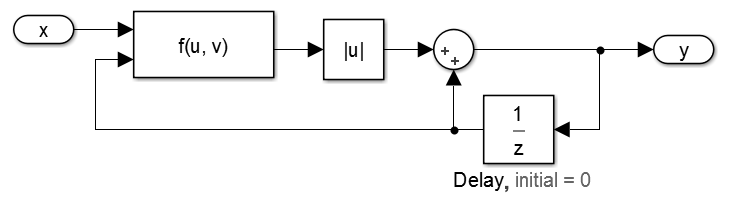
\includegraphics[width=\columnwidth]{figs/simulink.png}
%{\smaller
%\begin{verbatim}
%node filter(x : real) returns (a, b, y : real);
%let
%  a = f(x, 0.0 -> pre y);
%  b = if a >= 0.0 then a else -a;
%  y = b + (0.0 -> pre y);
%tel;
%\end{verbatim}
%}
%\vspace{-0.1in}
%\caption{Model with property $y \geq 0$, before IVC analysis}
%\label{fig:ex-before}
%\end{figure} 
\chapter{Preliminaries}
\label{sec:background}
The idea of inductive validity cores is applicable to the context of symbolic model checking using inductive proof methods. The idea is, after proving the correctness of a given property, to extract a minimal portion of the system (model) necessary for the proof of the property. In other words, we would like to determine why the property is satisfied by the system. Since this information is obtained from the inductive proofs, we call it \emph{inductive} validity core. With minimal IVCs, we are able to abstract away the part of the system irrelevant to the proof of the property. This chapter mentions some background we need for a formal description of the IVC notion.

\section{Safety Verification}

Given a state space $U$, a transition system $(I,T)$ consists of an
initial state predicate $ I : U \to \bool $ and a transition step
predicate $ T : U \times U \to \bool $.
We define the notion of
reachability for $(I, T)$ as the smallest predicate $\reach : U \to
\bool$ which satisfies the following formulas:

\begin{gather*}
  \forall u.~ I(u) \Rightarrow \reach(u) \\
  \forall u, u'.~ \reach(u) \land T(u, u') \Rightarrow \reach(u')
\end{gather*}

A safety property $P : U \to \bool$ is a state predicate. A safety
property $P$ holds on a transition system $(I, T)$ if it holds on all
reachable states, i.e., $\forall u.~ \reach(u) \Rightarrow P(u)$,
written as $\reach \Rightarrow P$ for short. When this is the case, we
write $(I, T)\vdash P$.

For an arbitrary transition system $(I, T)$, computing reachability
can be very expensive or even impossible. Thus, we need a more
effective way of checking if a safety property $P$ is satisfied by the
system. The key idea is to over-approximate reachability. If we can
find an over-approximation that implies the property, then the
property must hold. Otherwise, the approximation needs to be refined.

A good first approximation for reachability is the property itself.
That is, we can check if the following formulas hold:
\begin{gather}
  \forall u.~ I(u) \Rightarrow P(u)
  \label{eq:1-ind-base} \\
  \forall u, u'.~ P(u) \land T(u, u') \Rightarrow P(u')
  \label{eq:1-ind-step}
\end{gather}
If both formulas hold then $P$ is {\em inductive} and holds over the
system. If (\ref{eq:1-ind-base}) fails to hold, then $P$ is violated
by an initial state of the system. If (\ref{eq:1-ind-step}) fails to
hold, then $P$ is too much of an over-approximation and needs to be
refined.

One way to refine our over-approximation is to add additional lemmas
to the property of interest. For example, given another property $L :
U \to bool$ we can consider the extended property $P'(u) = P(u) \land
L(u)$, written as $P' = P \land L$ for short. If $P'$ holds on the
system, then $P$ must hold as well. The hope is that the addition of
$L$ makes formula (\ref{eq:1-ind-step}) provable because the
antecedent is more constrained. However, the consequent of
(\ref{eq:1-ind-step}) is also more constrained, so the lemma $L$ may
require additional lemmas of its own. Finding and proving these
lemmas is the means by which property directed reachability (PDR)
strengthens and proves a safety property~\cite{Een2011:PDR}.

Another way to refine our over-approximation is to use use {\em
  $k$-induction} which unrolls the property over $k$ steps of the
transition system. For example, 1-induction consists of formulas
(\ref{eq:1-ind-base}) and (\ref{eq:1-ind-step}) above, whereas
2-induction consists of the following formulas:
\begin{gather*}
\forall u.~ I(u) \Rightarrow P(u) \\
\forall u, u'.~ I(u) \land T(u, u') \Rightarrow P(u') \\
\forall u, u', u''.~ P(u) \land T(u, u') \land P(u') \land T(u',
  u'') \Rightarrow P(u'')
\end{gather*}
That is, there are two base step checks and one inductive step check.
In general, for an arbitrary $k$, $k$-induction consists of $k$
base step checks and one inductive step check as shown in
Figure~\ref{fig:k-induction} (the universal quantifiers on $u_i$ have
been elided for space). We say that a property is $k$-inductive if it
satisfies the $k$-induction constraints for the given value of $k$.
The hope is that the additional formulas in the antecedent of the
inductive step make it provable.

\begin{figure}
\begin{gather*}
I(u_0) \Rightarrow P(u_0) \\[-2pt]
%
\vdots \\[2pt]
%
I(u_0) \land T(u_0, u_1) \land \cdots \land T(u_{k-2}, u_{k-1})
\Rightarrow P(u_{k-1}) \\[2pt]
%
P(u_0) \land T(u_0, u_1) \land \cdots \land P(u_{k-1}) \land
T(u_{k-1}, u_k) \Rightarrow P(u_k)
\end{gather*}
\caption{$k$-induction formulas: $k$ base cases and one inductive
  step}
\label{fig:k-induction}
\end{figure}

In practice, inductive model checkers often use a combination of the
above techniques. Thus, a typical conclusion is of the form ``$P$ with
lemmas $L_1, \ldots, L_n$ is $k$-inductive''.


%%% Local Variables:
%%% mode: latex
%%% TeX-master: "main.tex"
%%% End

%%  LocalWords:  bool reachability JKind Lustre PDR Yices MathSAT ok
%%  LocalWords:  SMTInterpol dataflow init

\chapter{Proposed Approach}
% % \input{RelatedWork}
% % \input{ModelDevelopment}
% % \input{Discussion}
%\chapter{Conclusions}
  
In this proposal, we introduce the idea of extracting a minimal IVC for a given property and its applications.  However, a single IVC often does not provide a complete picture of the traceability from a property to a model.  We would also like to address the problem of extracting {\em all minimal} IVCs. 
We will show
the correctness and completeness of our methods and algorithms.  In addition, we plan to have a substantial evaluation that shows that the practicality and efficiency of our technique. For this purpose, we have collected a large set of benchmarks from different sources. Our experiments are conducted on a set of benchmarks containing 660 Lustre models, 530 from~\cite{Hagen08:FMCAD, piskac2016} and 130 industrial models derived from \cite{hilt2013} and other sources \cite{piskac2016, NFM2015:backes}.  Most of the academic benchmark models are small (10kB or less, with 6-40 equations) and include a range of hardware benchmarks and software problems involving counters that are difficult to solve inductively.
The industrial models are much larger; for example, each 80 models from \cite{hilt2013} contain over 600 equations and are each $\geq$80kB in size. The benchmark includes 2 models from NASA Quad-redundant Flight Control System (QFCS)~\cite{NFM2015:backes}: the Flight Control System (FCS) with 5259 Lustre equations and the Flight Control Computer (FCC) with 10969 equations.

We selected only benchmark problems consisting of a Lustre model with
properties that JKind could prove with a 3-hour timeout.
Experiments are run in a configuration with the \texttt{Z3} solver and the ``fastest'' mode of JKind (which involves running the $k$-induction and PDR engines in parallel and terminating when a solution is found). The experiments are expected to be run on an  Intel(R) i5-4690, 3.50GHz, 16 GB memory machine running Linux, and available online.

Our method for computing all MIVCs is inspired by a recent work in the domain of satisfiability analysis \cite{marco2016fast}. One interesting future direction is to devise similar MIVC enumeration algorithms based on other studies on MUSes extraction such as \cite{nadel2014accelerated}. 
Another interesting direction for this project is to parallelize the enumeration process: it is certainly possible to ask for multiple distinct maximal models to be solved in parallel.
%, though this may result in unnecessary work performed by some of the parallel solvers.

We also plan to investigate additional applications of the idea.  When performing {\em compositional verification}, the All-IVCs technique may be able to determine {\em minimal component sets} within an architecture that can satisfy a given set of requirements, which may be helpful for design-space exploration and synthesis. Finally, we are interested in adapting the notion of (all) validity cores for \emph{bounded} model checking for quantifying how much of models have been explored by bounded analysis.

Upon completion of the proposed research, we will have our IVCs computation algorithms integrated in the JKind model checker. The implementation will be benchmarked and evaluated rigorously. The usefulness of the IVC idea will be shown by utilizing its applications into different projects.


% \printglossary[title={LIST OF TERMS}, toctitle={List of Terms}]

%%%%%%%%%%%%%%%%%%%%%%%%%%%%%%%%%%%%%%%%%%%%%%%%%%%%%%%%%%%%%%%%%%%%%%%%%%%%%%%%
% WORKS CITED
%%%%%%%%%%%%%%%%%%%%%%%%%%%%%%%%%%%%%%%%%%%%%%%%%%%%%%%%%%%%%%%%%%%%%%%%%%%%%%%%
% When you need a works cited section, uncomment this and update the name of the
%   file.
%%%
    \bibliographystyle{abbrv}
%     \bibliographystyle{abbrvnat}
\bibliography{noAbbreviations,citations}


%%%%%%%%%%%%%%%%%%%%%%%%%%%%%%%%%%%%%%%%%%%%%%%%%%%%%%%%%%%%%%%%%%%%%%%%%%%%%%%%
% APPENDICIES
%%%%%%%%%%%%%%%%%%%%%%%%%%%%%%%%%%%%%%%%%%%%%%%%%%%%%%%%%%%%%%%%%%%%%%%%%%%%%%%%
% If you need an appendix, uncomment the following lines and add sections.
%%%
%\appendix
%\input{sectionName}

\end{document}
